\documentclass[aspectratio=169]{beamer}

% --- THEME AND COLOR ---
\usetheme{Madrid}
\usecolortheme{dolphin}

\makeatletter
\setbeamertemplate{footline}
{
  \leavevmode%
  \hbox{%
  \begin{beamercolorbox}[wd=.333333\paperwidth,ht=2.25ex,dp=1ex,center]{author in head/foot}%
    \usebeamerfont{author in head/foot}\insertshortauthor
  \end{beamercolorbox}%
  \begin{beamercolorbox}[wd=.333333\paperwidth,ht=2.25ex,dp=1ex,center]{title in head/foot}%
    \usebeamerfont{title in head/foot}\insertshorttitle
  \end{beamercolorbox}%
  \begin{beamercolorbox}[wd=.333333\paperwidth,ht=2.25ex,dp=1ex,right]{date in head/foot}%
    \usebeamerfont{date in head/foot}\insertshortdate{}\hspace*{2em}
    \insertframenumber{} / \inserttotalframenumber\hspace*{2ex} 
  \end{beamercolorbox}}%
  \vskip0pt%
}
\makeatother
\setbeamertemplate{navigation symbols}{}

% --- PACKAGES ---
\usepackage[utf8]{inputenc}
\usepackage[T1]{fontenc}
\usepackage{amsmath,amssymb,graphicx,booktabs,hyperref,siunitx,multirow}
\hypersetup{colorlinks=true,linkcolor=blue,urlcolor=blue}
\graphicspath{{images/}}

% --- PRESENTATION METADATA ---
\title[CFD Assignments]{CLL769: Applications of CFD \\ Assignments 1, 2, 5 \& 6}
\subtitle{Pipe Flow, Cylinder Wake, Fluidized Beds, \& Bubble Rise}
\author[Sajeev]{Sajeev}
\institute[]{Department of Chemical Engineering, IIT Delhi}
\date{}

% --- IIT DELHI LOGO ---
\titlegraphic{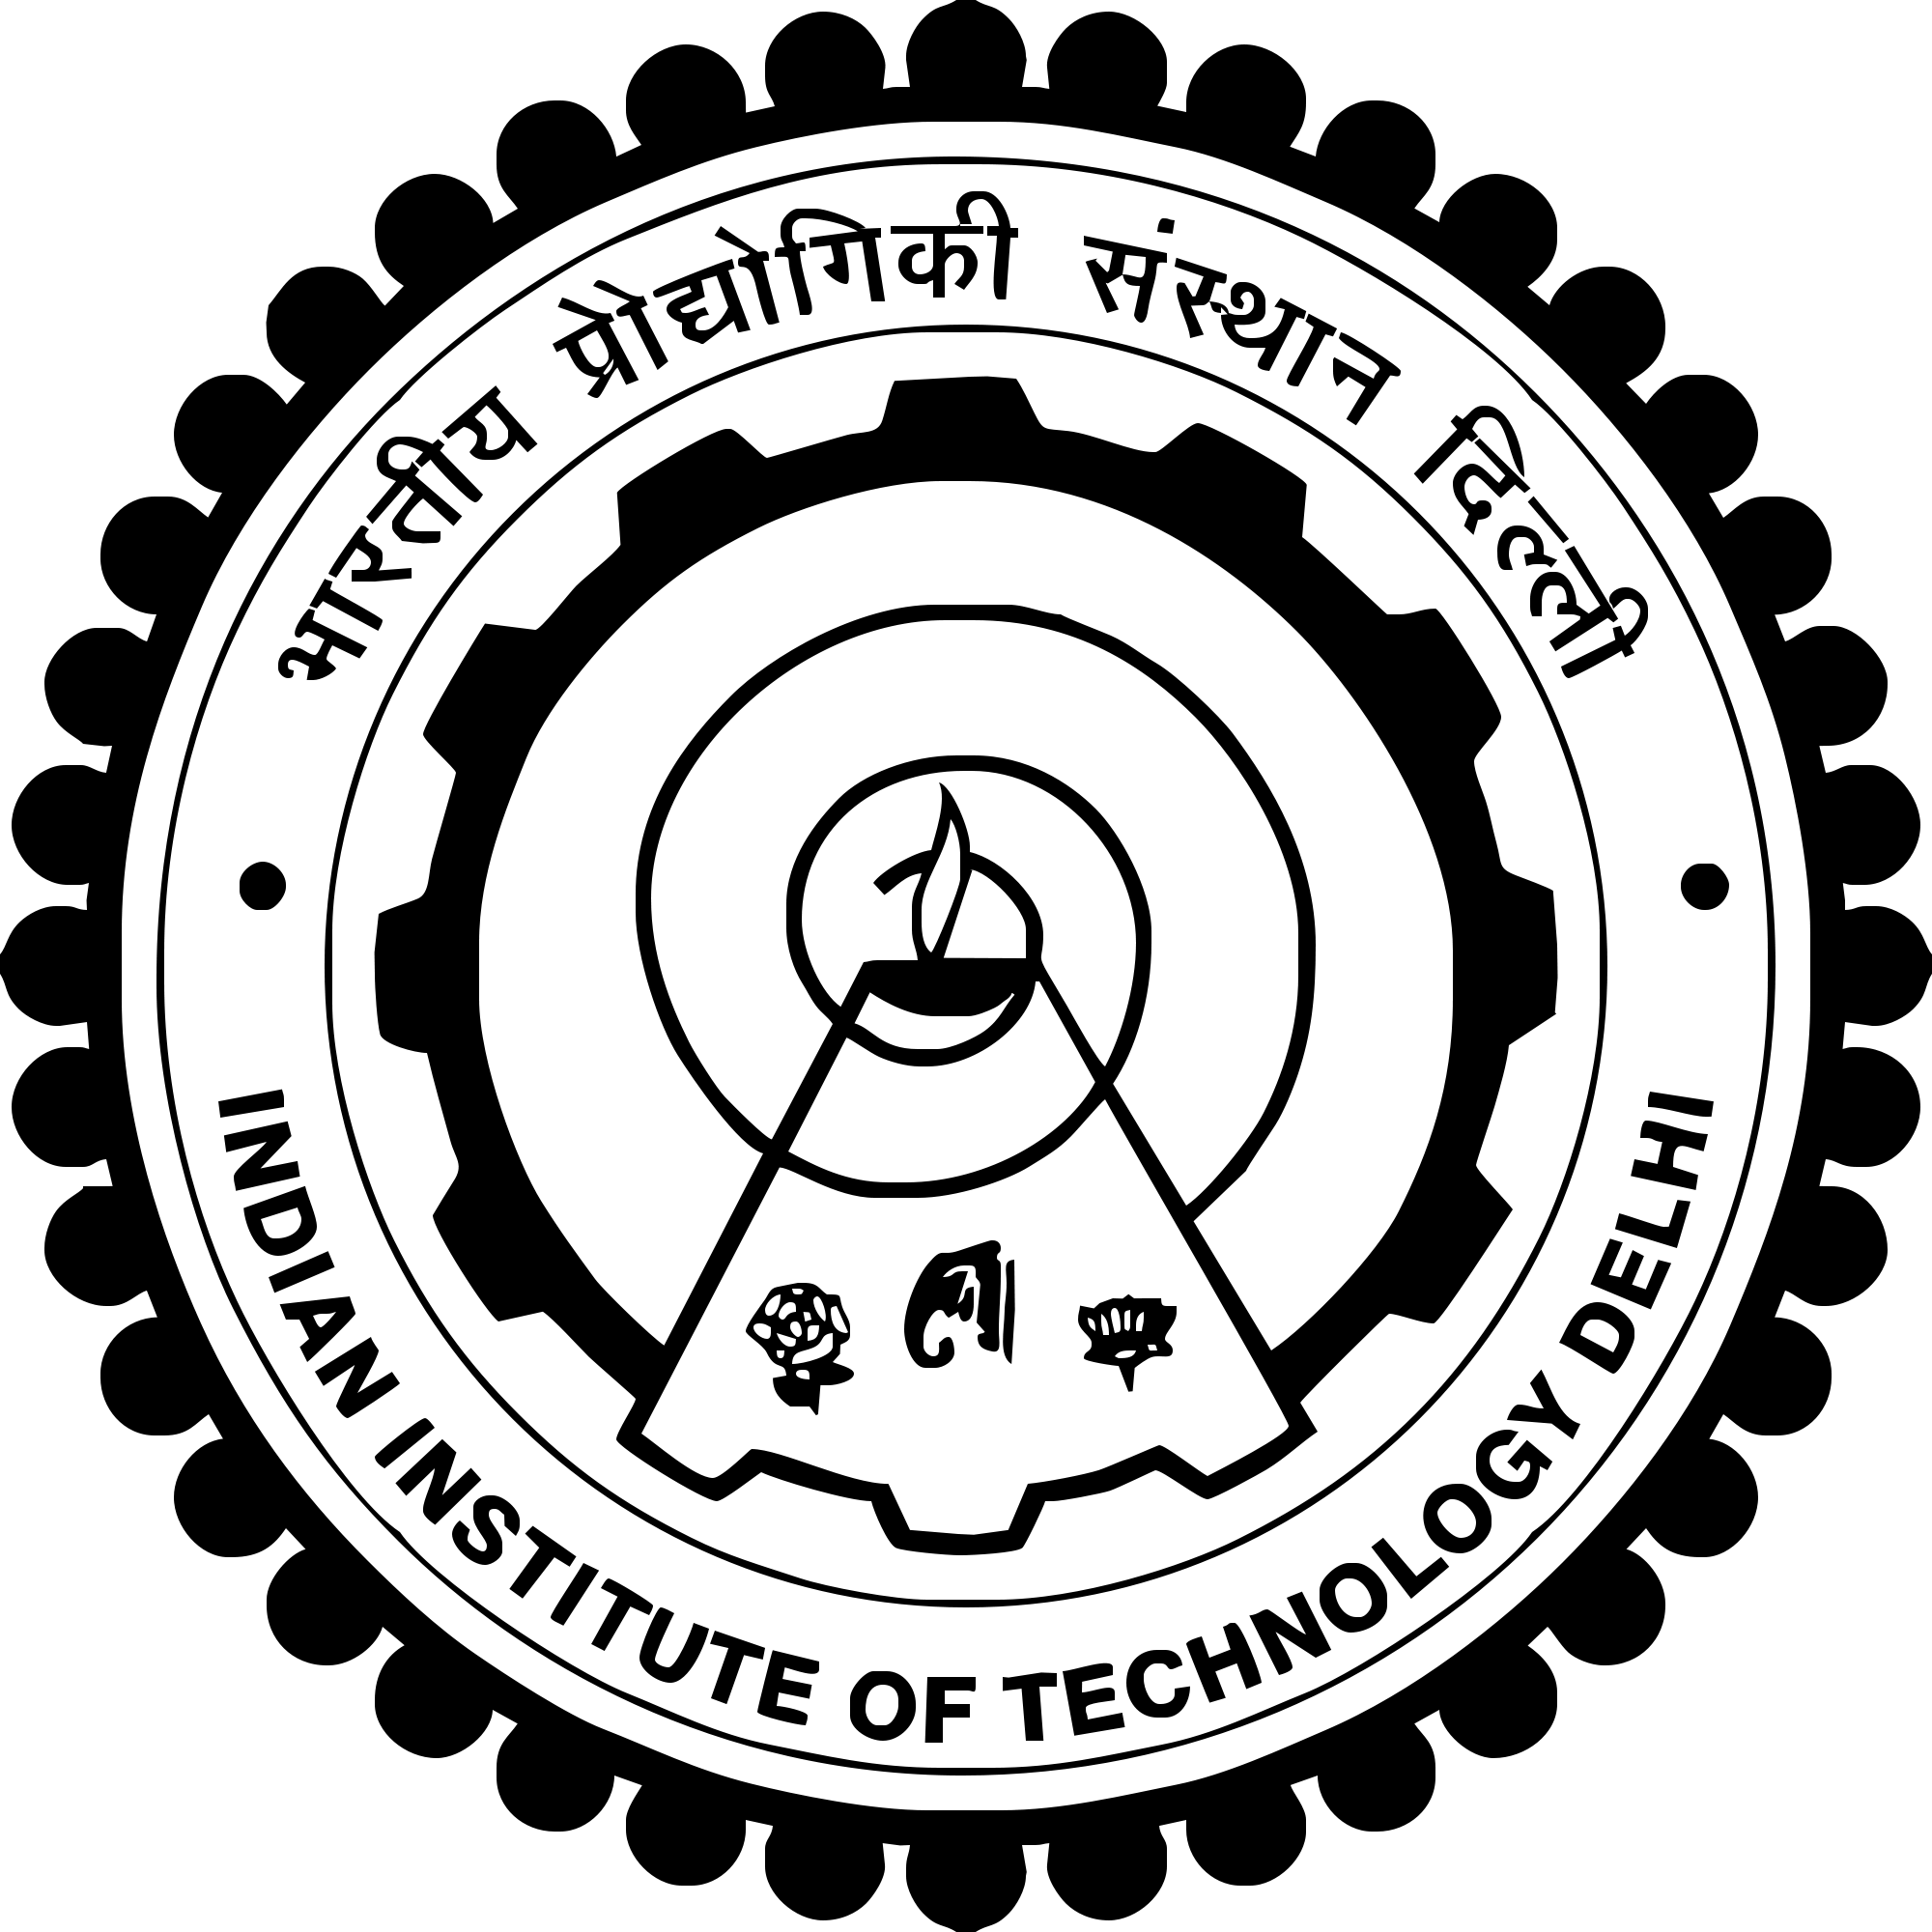
\includegraphics[width=2cm]{iitd_logo.png}}

\newcommand{\bi}{\begin{itemize}}
\newcommand{\ei}{\end{itemize}}
\newcommand{\ben}{\begin{enumerate}}
\newcommand{\een}{\end{enumerate}}
\newcommand{\im}{\item}

\begin{document}

\begin{frame}
    \maketitle
\end{frame}

\begin{frame}{Outline}
    \tableofcontents
\end{frame}

% --- TUTORIAL 1 START ---
\section{Tutorial 1: Pipe Flow}
\begin{frame}
    \centering \Huge \textbf{Tutorial 1: Pipe Flow}
\end{frame}

\begin{frame}{Problem Statement \& Objective}
    \begin{block}{Objective}
    Perform numerical simulations of a steady, laminar flow of a Newtonian, incompressible fluid in a pipe.
    \end{block}
    \vspace{0.3cm}
    \begin{block}{System Details}
    \bi
        \im \textbf{Geometry:} Pipe of length $1$ m and radius $0.1$ m.
        \im \textbf{Flow Regime:} Laminar, $Re = 100$.
        \im \textbf{Analysis:} Axisymmetric 2D simulation.
    \ei
    \end{block}
\end{frame}

% --- SECTION 2 ---
\section{Governing Equations}
\begin{frame}{Governing Equations}
    The flow is governed by the steady-state, incompressible Navier-Stokes equations for a Newtonian fluid.

    \begin{block}{Continuity Equation}
    \[
    \nabla \cdot \vec{U} = 0
    \]
    \end{block}
    
    \begin{block}{Momentum Equation (Navier-Stokes)}
    \[
    \rho (\vec{U} \cdot \nabla) \vec{U} = -\nabla P + \mu \nabla^2 \vec{U}
    \]
    \end{block}
\end{frame}

% --- SECTION 3 ---
\section{Computational Setup}
\begin{frame}{Computational Setup \& Boundary Conditions}
    \begin{columns}[T]
        \begin{column}{0.5\textwidth}
            \begin{block}{Boundary Conditions}
            \bi
                \im \textbf{Inlet:} Velocity inlet.
                \im \textbf{Outlet:} Pressure outlet (0 gauge).
                \im \textbf{Top Edge:} Wall (No-slip condition).
                \im \textbf{Bottom Edge:} Axis of symmetry.
            \ei
            \end{block}
            \begin{block}{Physical Properties}
            To achieve $Re = \frac{\rho U D}{\mu} = 100$:
            \bi
                \im Diameter $D = 0.2$ m
                \im e.g., $\rho = 1$ kg/m$^3$, $U = 0.5$ m/s, $\mu = 0.001$ kg/m-s.
            \ei
            \end{block}
        \end{column}
        \begin{column}{0.48\textwidth}
            \begin{block}{Numerical Schemes}
            \bi
                \im \textbf{Solver:} Pressure-based, Steady, Axisymmetric.
                \im \textbf{P-V Coupling:} SIMPLE algorithm.
                \im \textbf{Spatial Discretization:} QUICK scheme for momentum.
                \im \textbf{Convergence Criteria:} Normalized residuals $< 1 \times 10^{-6}$ for all variables.
            \ei
            \end{block}
        \end{column}
    \end{columns}
\end{frame}

\begin{frame}{Geometry \& Meshing}
    \begin{columns}[c]
        \begin{column}{0.48\textwidth}
            \textbf{Mesh Details:}
            \bi
                \im An axisymmetric 2D structured mesh was created for the pipe.
                \im A bias factor was applied towards the wall to adequately resolve the velocity gradients in the boundary layer.
            \ei
        \end{column}
        \begin{column}{0.48\textwidth}
            \centering
            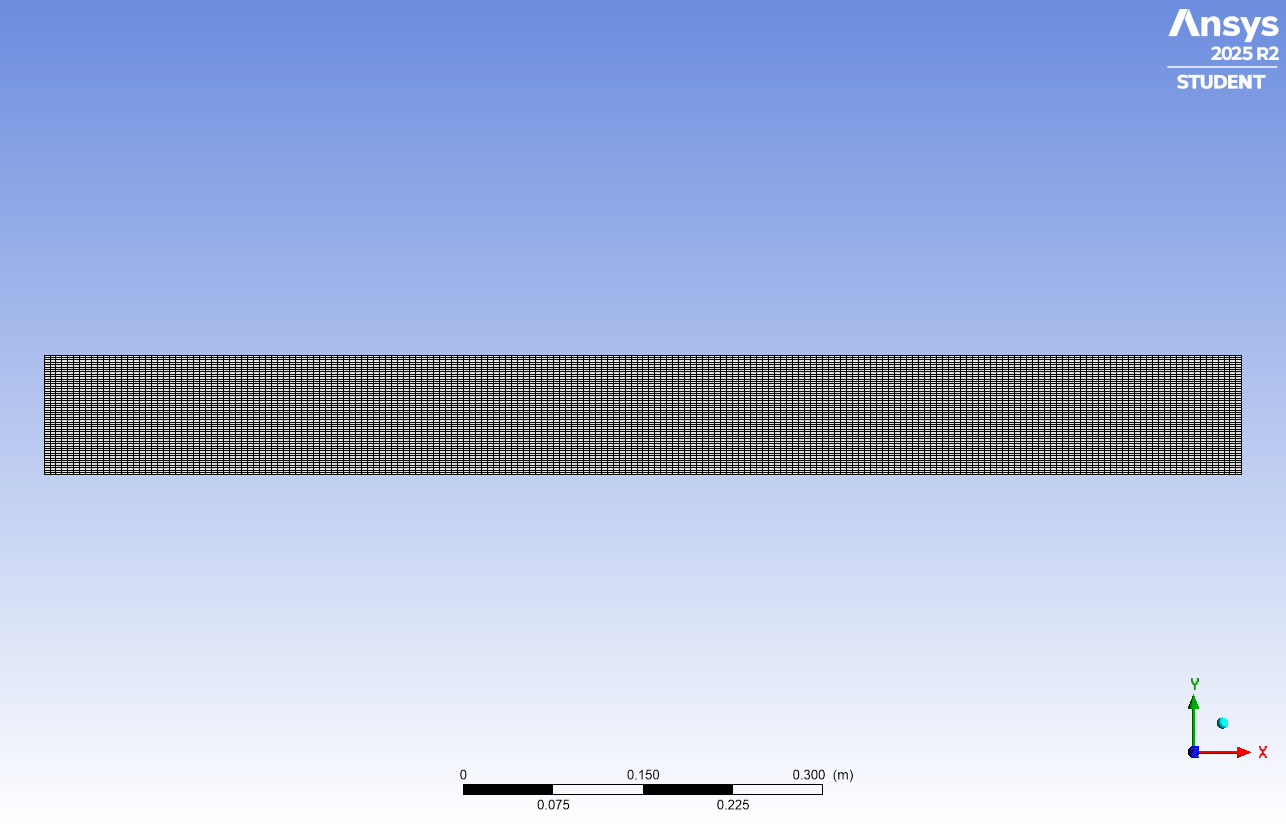
\includegraphics[width=\linewidth,height=0.6\textheight,keepaspectratio]{tut1_mesh.png}\\
            \vspace{0.2cm}
            {\scriptsize \textit{Representative view of the computational grid.}}
        \end{column}
    \end{columns}
\end{frame}

% --- SECTION 4 ---
\section{Results}
\begin{frame}{Velocity Distribution (Vector \& Contour)}
    \begin{columns}[c]
        \begin{column}{0.48\textwidth}
            \centering
            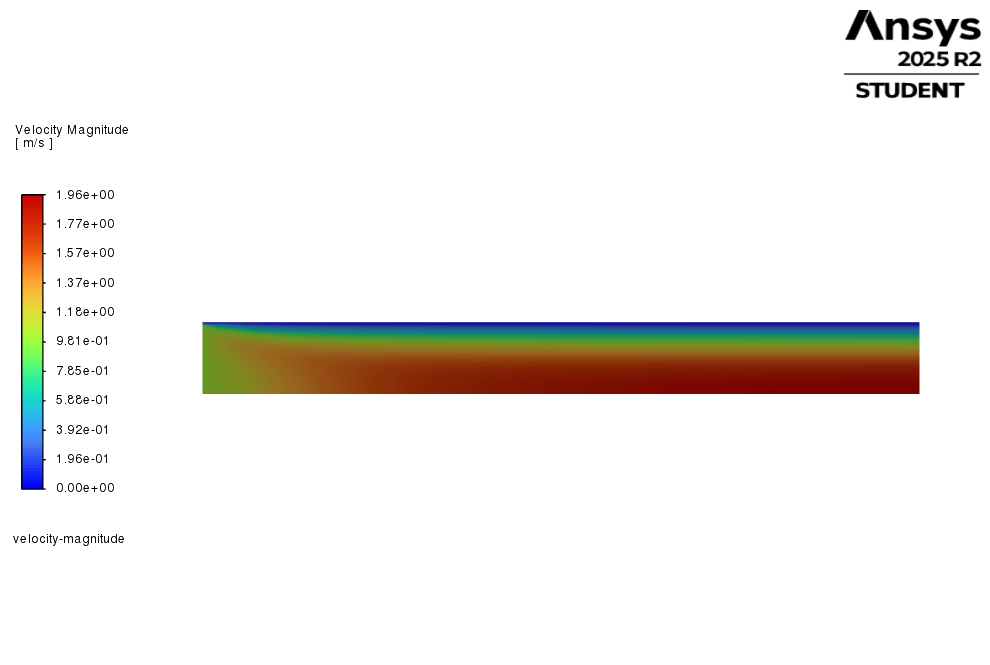
\includegraphics[width=\linewidth,height=0.45\textheight,keepaspectratio]{tut1_vel_cont.png}\\
            \vspace{0.1cm}
            {\scriptsize \textit{Velocity magnitude contour.}}
        \end{column}
        \begin{column}{0.48\textwidth}
            \centering
            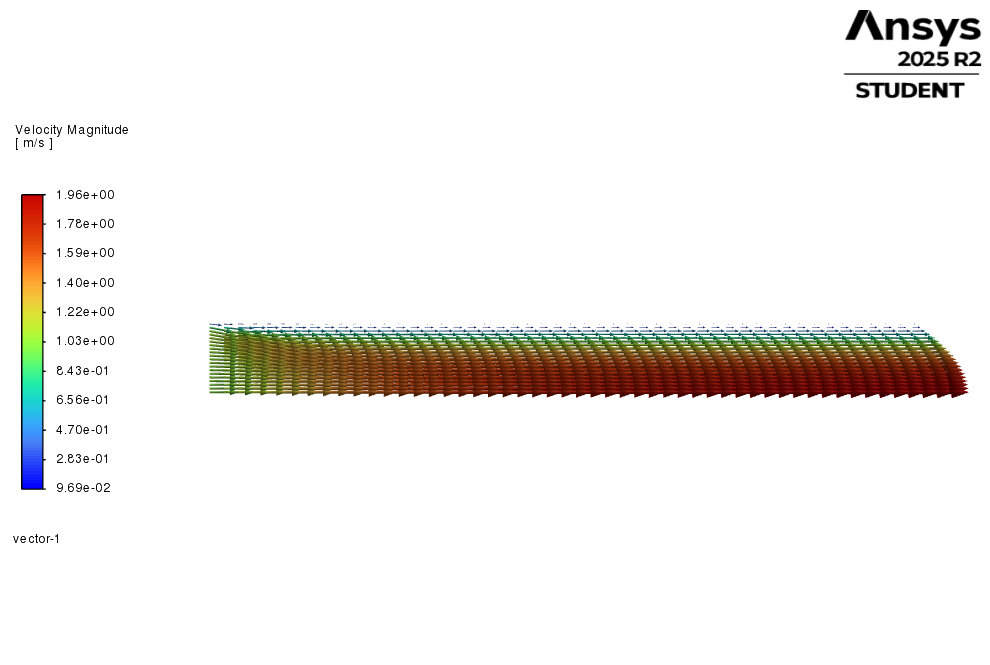
\includegraphics[width=\linewidth,height=0.45\textheight,keepaspectratio]{tut1_vel_vect.png}\\
            \vspace{0.1cm}
            {\scriptsize \textit{Velocity vectors colored by magnitude.}}
        \end{column}
    \end{columns}
    \vspace{0.3cm}
    \begin{block}{Observations}
    The flow enters with a uniform velocity and gradually develops into a parabolic profile. The maximum velocity occurs at the axis (bottom edge), and zero velocity at the wall (top edge) due to the no-slip condition.
    \end{block}
\end{frame}

\begin{frame}{Validation: Velocity Profile \& Pressure Drop}
    \begin{columns}[c]
        \begin{column}{0.48\textwidth}
            \centering
            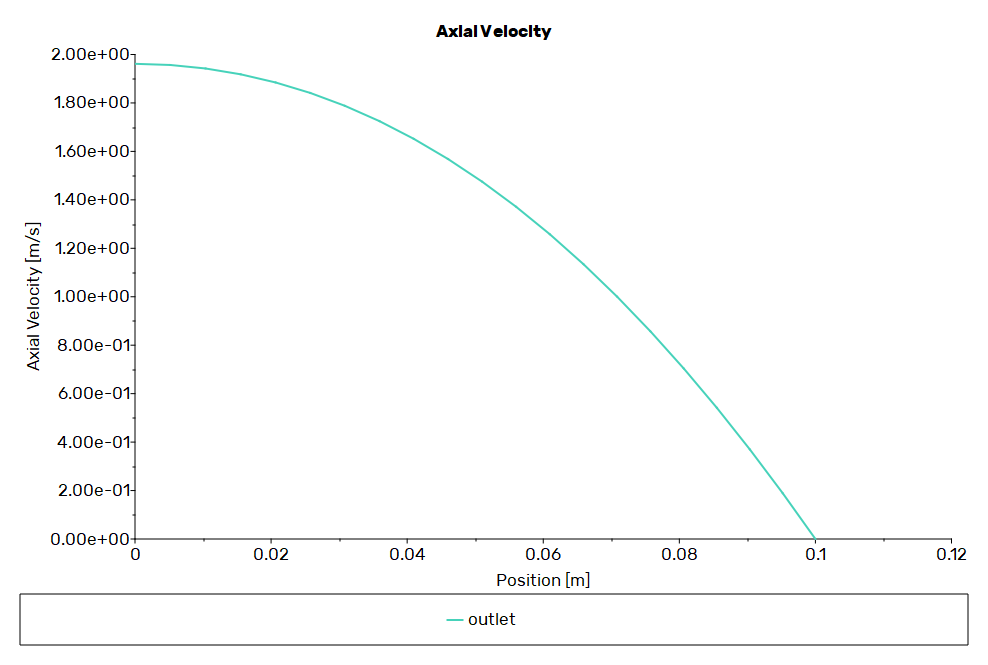
\includegraphics[width=0.48\linewidth,height=0.55\textheight,keepaspectratio]{tut1_vel_prof.png}
            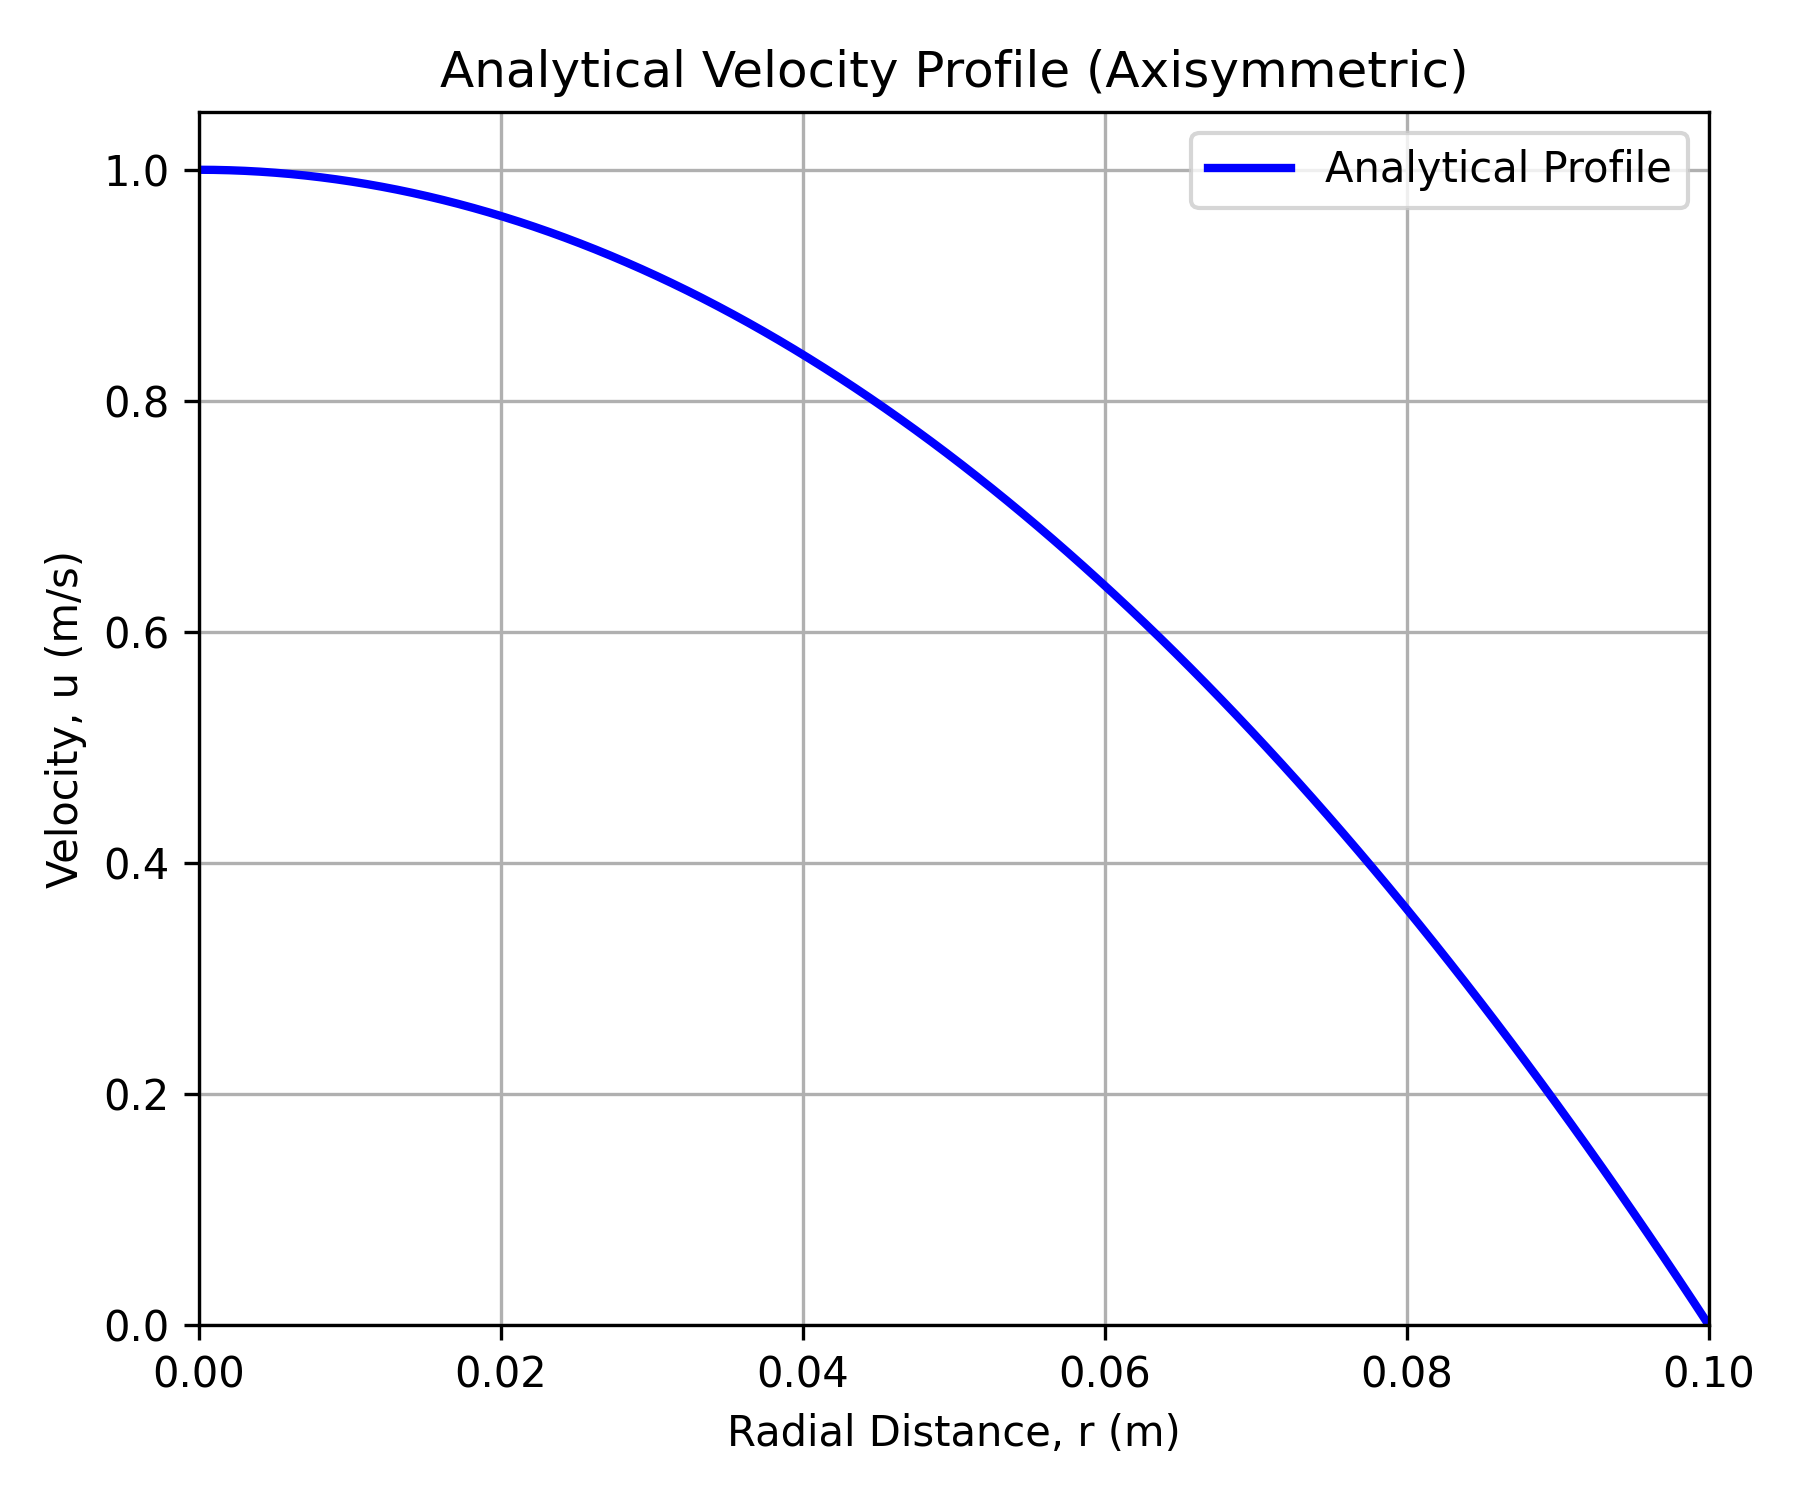
\includegraphics[width=0.48\linewidth,height=0.55\textheight,keepaspectratio]{tut1_vel_prof_analytical.png}\\
            \vspace{0.1cm}
            {\scriptsize \textit{Left: Simulated. Right: Analytical Profile.}}
        \end{column}
        \begin{column}{0.48\textwidth}
            \begin{block}{Velocity Profile}
            \small
            The predicted fully developed profile matches the analytical solution perfectly:
            \[
            u(r) = 2(0.5) \left( 1 - \left(\frac{r}{0.1}\right)^2 \right) = 1.0\left( 1 - 100r^2 \right) \text{ m/s}
            \]
            \end{block}
            \begin{block}{Pressure Drop}
            \small
            The linear pressure drop matches the Hagen-Poiseuille equation:
            \[
            \frac{\Delta P}{L} = \frac{8 \mu U_{\text{avg}}}{R^2} = \frac{8 (0.001) (0.5)}{(0.1)^2} = 0.4 \text{ Pa/m}
            \]
            The simulated pressure drop matches this calculated analytical value of $0.4$ Pa/m exactly.
            \end{block}
        \end{column}
    \end{columns}
\end{frame}

\begin{frame}{Wall Shear Stress}
    \begin{columns}[c]
        \begin{column}{0.5\textwidth}
            \centering
            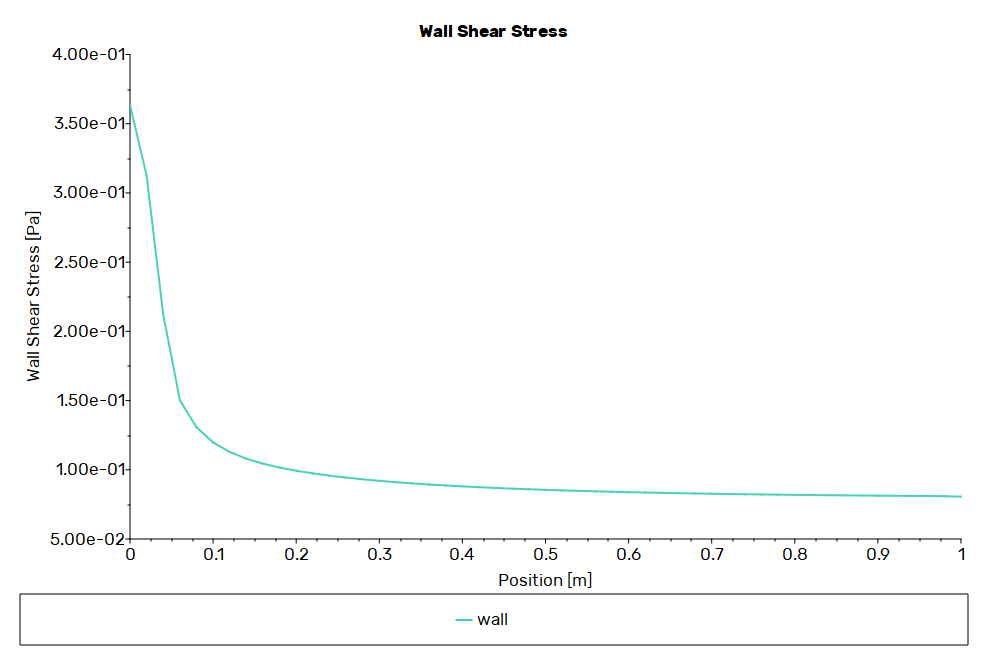
\includegraphics[width=\linewidth,height=0.6\textheight,keepaspectratio]{tut1_wall_shear.png}\\
            \vspace{0.1cm}
            {\scriptsize \textit{Variation of wall shear stress along the pipe length.}}
        \end{column}
        \begin{column}{0.48\textwidth}
            \begin{block}{Hydrodynamic Entrance Region}
            \bi
                \im Near the inlet ($x=0$), the velocity gradient at the wall is extremely steep, resulting in high wall shear stress.
                \im As the boundary layer grows and the flow develops, the wall shear stress decreases exponentially.
                \im The stress reaches a constant horizontal asymptote once the flow is \textbf{fully developed}.
            \ei
            \end{block}
        \end{column}
    \end{columns}
\end{frame}



% --- TUTORIAL 2 START ---
\section{Tutorial 2: Flow Over a Cylinder}
\begin{frame}
    \centering \Huge \textbf{Tutorial 2: Flow Over a Cylinder}
\end{frame}
\begin{frame}{Problem Statement \& Objective}
    \begin{block}{Objective}
    Perform 2D numerical simulations of unsteady flow of a Newtonian, incompressible fluid over a cylinder to study vortex shedding.
    \end{block}
    \vspace{0.3cm}
    \begin{block}{System Details}
    \bi
        \im \textbf{Geometry:} Pipe of $15 \times 5$ m with a cylinder of diameter $D=1$ m located 5 m from the inlet.
        \im \textbf{Flow Regimes:} Laminar ($Re = 272$) and Turbulent ($Re = 2902$).
        \im \textbf{Fluid Properties:} $U = 0.5$ m/s, $\rho = 1$ kg/m$^3$. Viscosity adjusted for Re.
    \ei
    \end{block}
\end{frame}

\begin{frame}{Computational Setup}
    \begin{columns}[T]
        \begin{column}{0.5\textwidth}
            \begin{block}{Boundary Conditions}
            \bi
                \im \textbf{Inlet:} Velocity inlet ($0.5$ m/s).
                \im \textbf{Outlet:} Pressure outlet (0 gauge).
                \im \textbf{Walls \& Cylinder:} No-slip condition.
            \ei
            \end{block}
            \begin{block}{Models}
            \bi
                \im \textbf{Laminar Case:} Laminar viscous model.
                \im \textbf{Turbulent Case:} Standard $k-\epsilon$ model.
            \ei
            \end{block}
        \end{column}
        \begin{column}{0.48\textwidth}
            \begin{block}{Numerical Schemes}
            \bi
                \im \textbf{Solver:} Pressure-based, Transient, Planar.
                \im \textbf{P-V Coupling:} SIMPLE algorithm.
                \im \textbf{Spatial Discretization:} QUICK for momentum.
                \im \textbf{Transient Formulation:} 2nd Order Implicit.
            \ei
            \end{block}
        \end{column}
    \end{columns}
\end{frame}

\begin{frame}{Geometry \& Meshing}
    \begin{columns}[c]
        \begin{column}{0.5\textwidth}
            \centering
            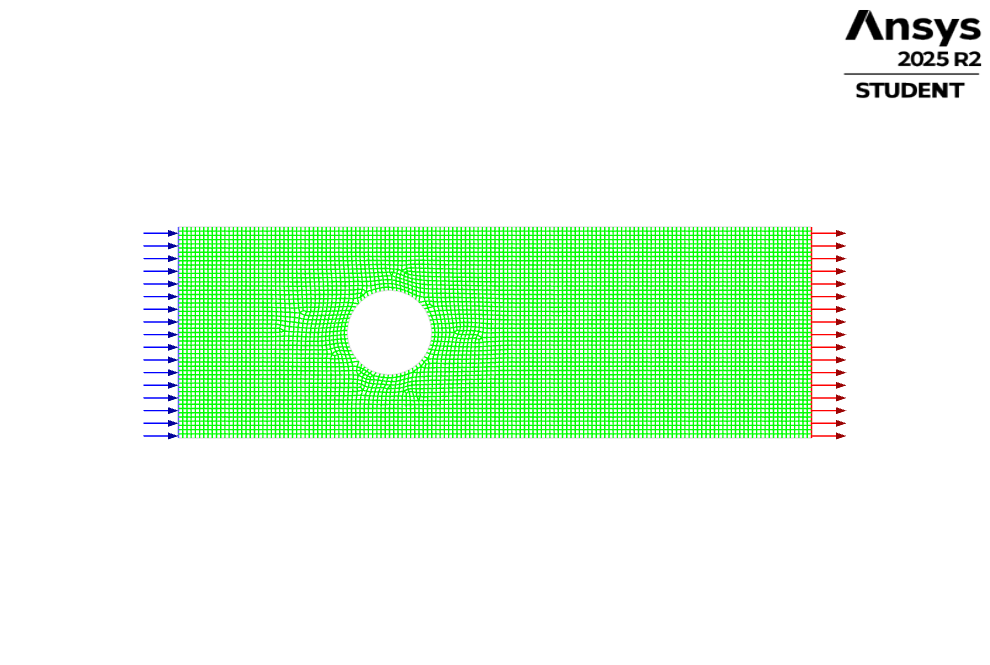
\includegraphics[width=\linewidth,height=0.6\textheight,keepaspectratio]{mesh.png}\\
            \vspace{0.2cm}
            {\scriptsize \textit{Computational grid around the cylinder.}}
        \end{column}
        \begin{column}{0.48\textwidth}
            \begin{block}{Mesh Details}
            \bi
                \im An unstructured mesh with inflation layers near the cylinder walls was generated.
                \im The grid is highly refined near the cylinder to capture the boundary layer separation and wake dynamics accurately.
                \im The far-field regions are slightly coarser to optimize computational cost.
            \ei
            \end{block}
        \end{column}
    \end{columns}
\end{frame}



\begin{frame}{Vortex Shedding Frequency}
    \begin{columns}[c]
        \begin{column}{0.48\textwidth}
            \centering
            \textbf{Laminar ($Re = 272$)}\\
            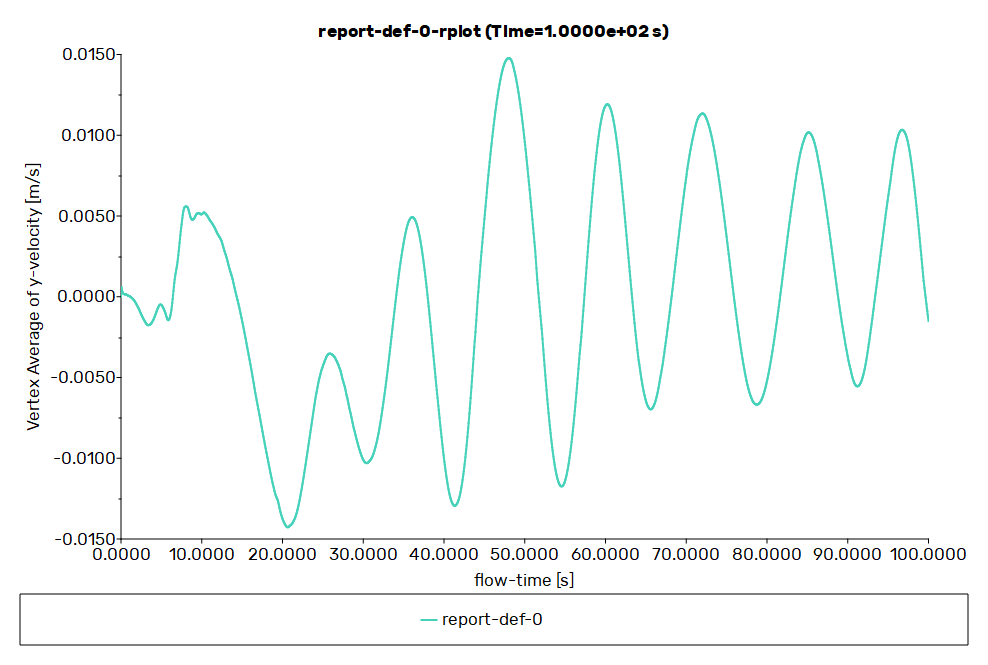
\includegraphics[width=\linewidth,height=0.4\textheight,keepaspectratio]{xy-272-2000.png}\\
            {\scriptsize \textit{$f \approx 0.105$ Hz.}}
        \end{column}
        \begin{column}{0.48\textwidth}
            \centering
            \textbf{Turbulent ($Re = 2902$)}\\
            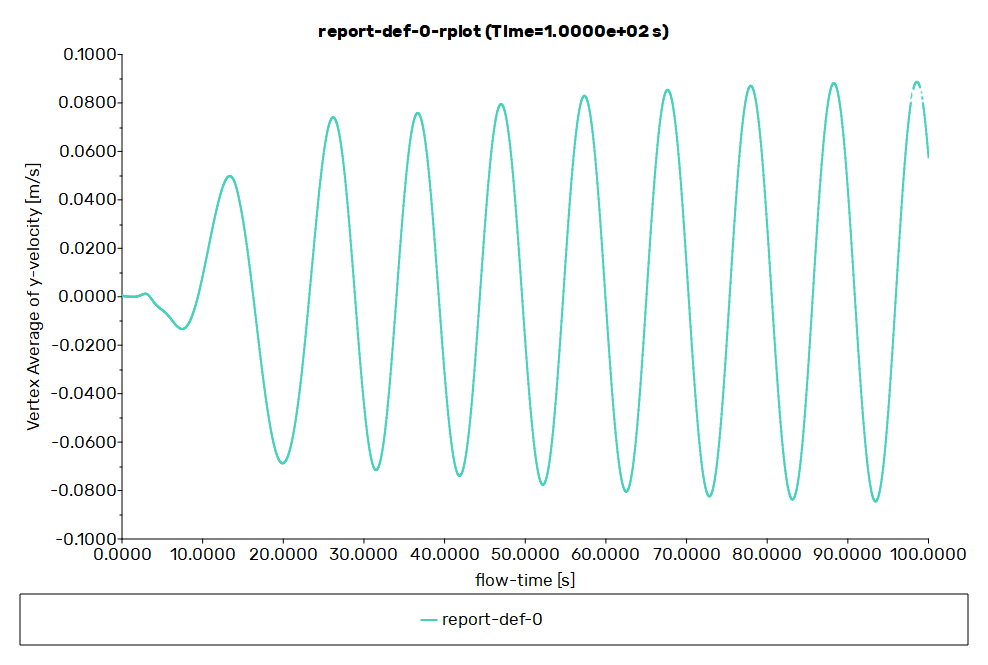
\includegraphics[width=\linewidth,height=0.4\textheight,keepaspectratio]{xy-2902-2000.png}\\
            {\scriptsize \textit{$f \approx 0.133$ Hz.}}
        \end{column}
    \end{columns}
    \vspace{0.2cm}
    \begin{block}{Frequency Analysis}
    The y-velocity at a point behind the cylinder was monitored. For the laminar case ($Re=272$), the oscillation period $T \approx 9.5$ s gives a shedding frequency $f \approx 0.105$ Hz. For the turbulent case ($Re=2902$), the $k-\epsilon$ model yields a faster oscillation with period $T \approx 7.5$ s and frequency $f \approx 0.133$ Hz.
    \end{block}
\end{frame}

\begin{frame}{Animation of the Vortex Street}
    \begin{block}{Transient Flow Visualization}
    A solution animation was recorded during the transient simulation to capture the dynamics of the wake formation and the vortex shedding process over time.
    \end{block}
    \vspace{0.3cm}
    \begin{center}
        \textit{(Please refer to the accompanying video file: \texttt{turbulent-vortex-video.mpeg})} \\
        \vspace{0.3cm}
        \textbf{Watch Animation:} \href{https://github.com/sajeev505/cll769_tuts_submission/blob/main/Tut_2/turbulent-vortex-video.mpeg}{Click here to view the video on GitHub!}
    \end{center}
\end{frame}

% --- TUTORIAL 5 START ---
\section{Tutorial 5: Gas-Solid Fluidized Bed}
\begin{frame}
    \centering \Huge \textbf{Tutorial 5: Gas-Solid Fluidized Bed}
\end{frame}
\begin{frame}{Problem Statement \& Objective}
    \begin{block}{Objective}
    Perform Eulerian Two-Fluid Model (TFM) simulations of gas-solid fluidization in a pseudo-2D rectangular bed to investigate bubbling dynamics.
    \end{block}
    \vspace{0.3cm}
    \begin{block}{System Details}
    \bi
        \im \textbf{Geometry:} Pseudo-2D domain ($0.2$ m $\times$ $1.0$ m $\times$ $0.02$ m).
        \im \textbf{Phases:} Primary: Air (gas). Secondary: Glass beads (solid, $d_p = 2.26$ mm, $\rho_s = 2600$ kg/m$^3$).
        \im \textbf{Inlet Gas Velocities:} $U_g = 1.736$ m/s and $U_g = 2.78$ m/s.
    \ei
    \end{block}
\end{frame}

\begin{frame}{Computational Setup \& Models}
    \begin{columns}[T]
        \begin{column}{0.5\textwidth}
            \begin{block}{Boundary Conditions}
            \bi
                \im \textbf{Inlet:} Velocity inlet for gas, $0$ m/s for solids.
                \im \textbf{Outlet:} Pressure outlet ($0$ Pa).
                \im \textbf{Walls:} No-slip (gas), Johnson-Jackson (solids) with specularity $0.05$.
            \ei
            \end{block}
            \begin{block}{Initial State}
            Static bed height of $0.2$ m patched with solid volume fraction $\alpha_s = 0.6$.
            \end{block}
        \end{column}
        \begin{column}{0.48\textwidth}
            \begin{block}{Multiphase \& KTGF Models}
            \bi
                \im \textbf{Eulerian Model:} 2 Phases, Phase-Coupled SIMPLE.
                \im \textbf{Drag:} Gidaspow Model.
                \im \textbf{Granular Properties:} Syamlal-O'Brien (radial), Lun-et-al (pressure), Schaeffer (friction).
                \im \textbf{Transient Scheme:} 2nd Order Implicit ($\Delta t = 0.001$ s).
            \ei
            \end{block}
        \end{column}
    \end{columns}
\end{frame}

\begin{frame}{Geometry \& Meshing}
    \begin{columns}[c]
        \begin{column}{0.5\textwidth}
            \centering
            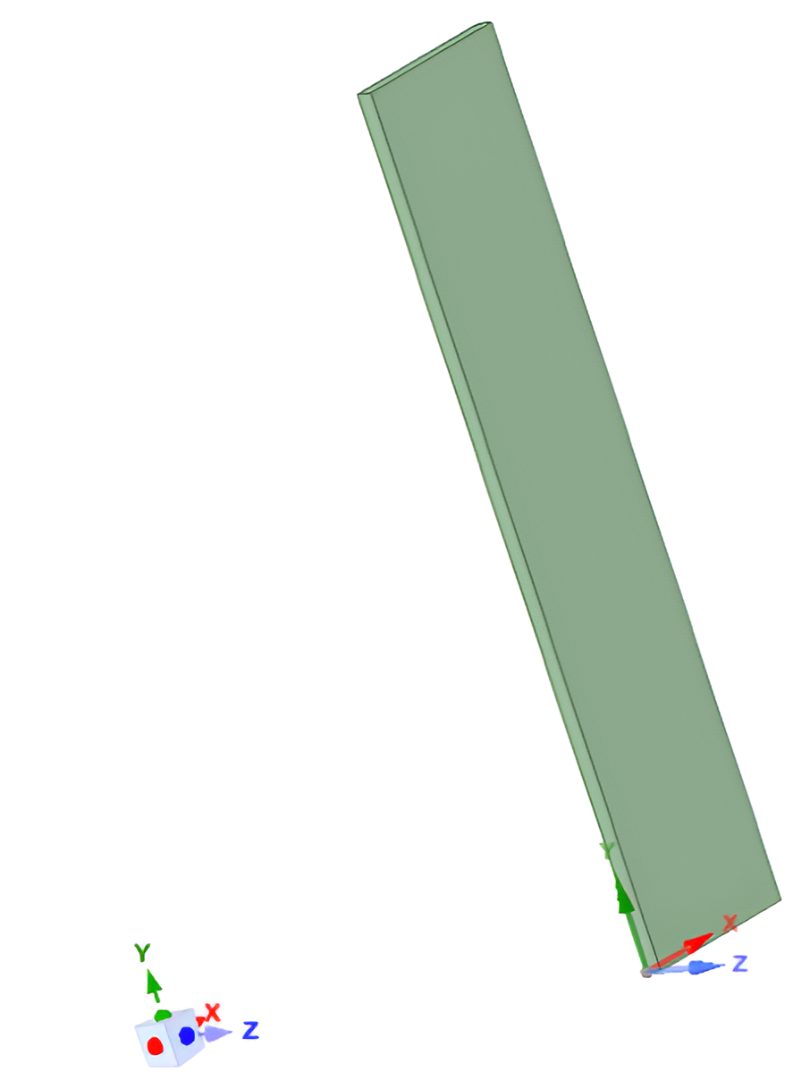
\includegraphics[width=0.6\linewidth,height=0.6\textheight,keepaspectratio]{tut5_geometry.png} \hspace{0.5cm}
            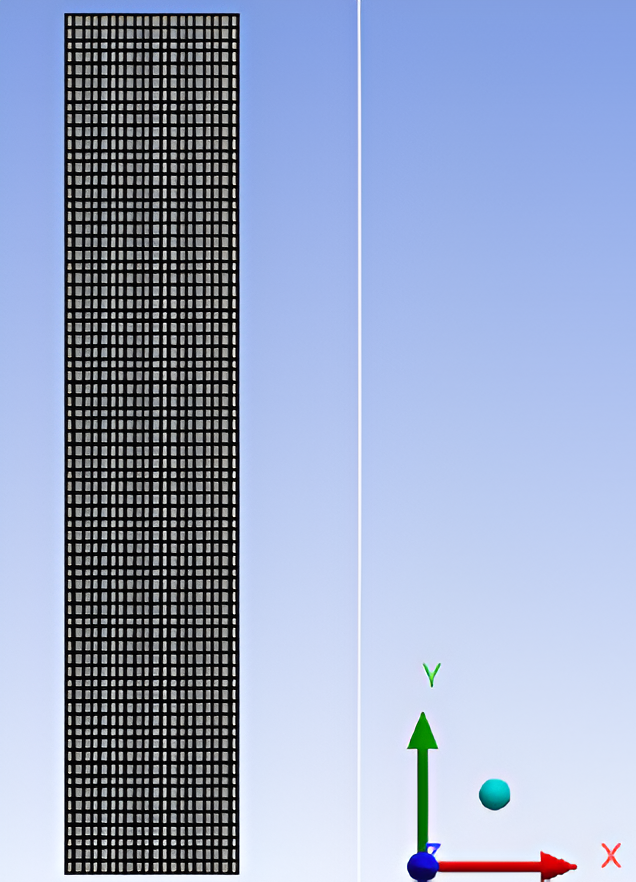
\includegraphics[width=0.3\linewidth,height=0.6\textheight,keepaspectratio]{tut5_mesh.png} \\
            \vspace{0.2cm}
            {\scriptsize \textit{Domain geometry and the $20 \times 70 \times 4$ uniform block-structured grid.}}
        \end{column}
        \begin{column}{0.48\textwidth}
            \begin{block}{Mesh Details}
            \bi
                \im A uniform structured grid of $5,600$ total cells.
                \im Resolution: $20$ divisions (width), $70$ divisions (height), and $4$ divisions (depth).
                \im Pseudo-2D setup balances accuracy for capturing mesoscale structures with computational efficiency.
            \ei
            \end{block}
        \end{column}
    \end{columns}
\end{frame}

\begin{frame}{Fluidization Dynamics: Solid Volume Fraction ($\alpha_s$)}
    \begin{columns}[c]
        \begin{column}{0.48\textwidth}
            \centering
            \textbf{$U_g = 1.736$ m/s} \\
            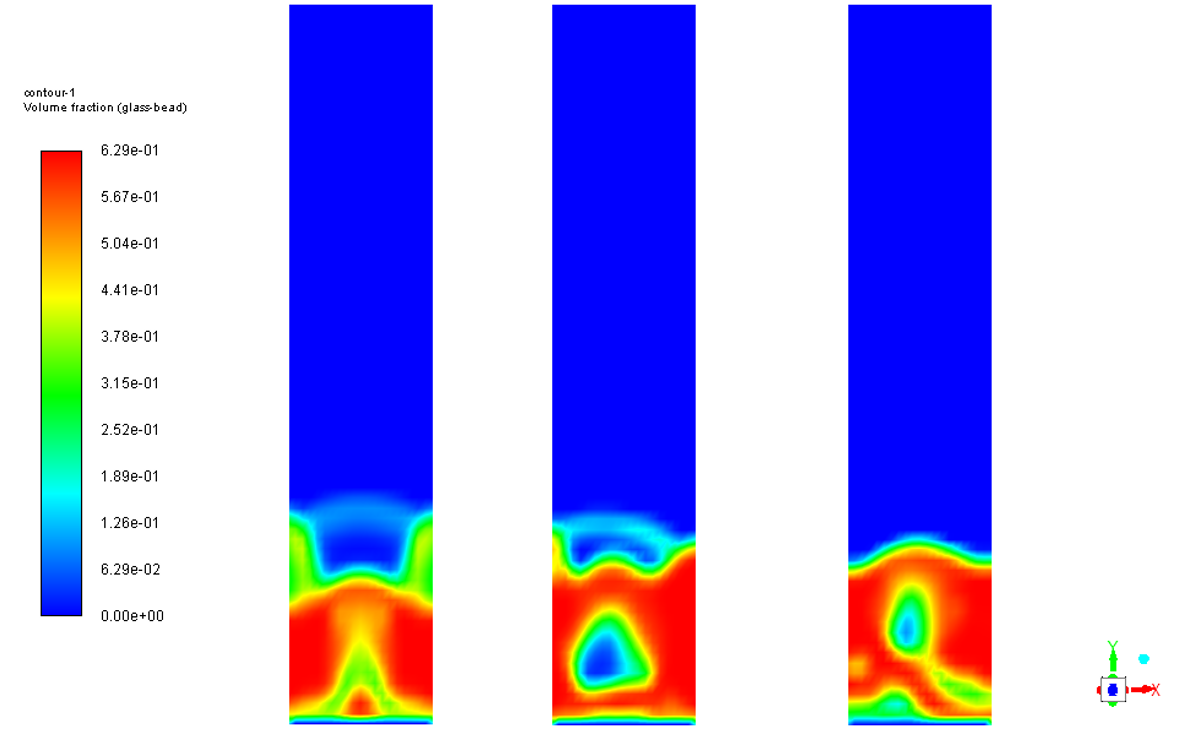
\includegraphics[width=0.9\linewidth,height=0.45\textheight,keepaspectratio]{volfrac_1_736.png}\\
            {\scriptsize \textit{Distinct, smaller bubbles rising through bed.}}
        \end{column}
        \begin{column}{0.48\textwidth}
            \centering
            \textbf{$U_g = 2.78$ m/s} \\
            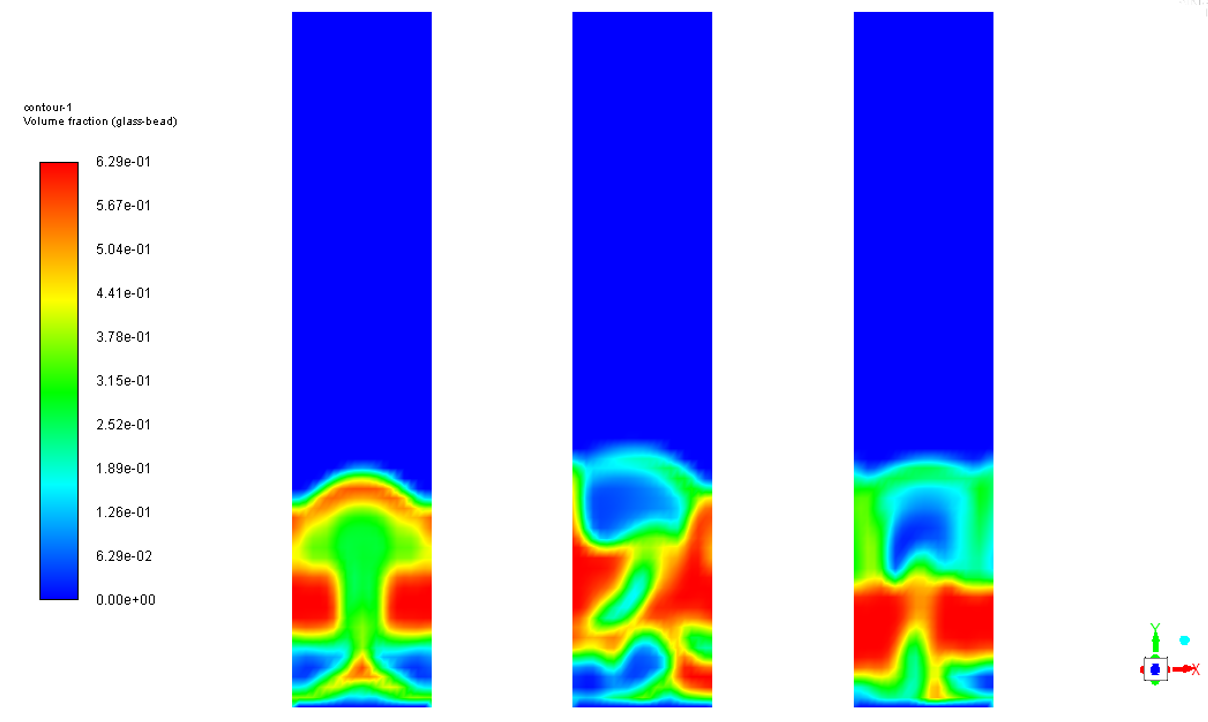
\includegraphics[width=0.9\linewidth,height=0.45\textheight,keepaspectratio]{volfrac_2_78.png}\\
            {\scriptsize \textit{Vigorous bubbling, distorted bubbles.}}
        \end{column}
    \end{columns}
    \vspace{0.3cm}
    \begin{block}{Comparison}
    At the higher superficial gas velocity, bubble formation is more intense. The bubbles are significantly larger, rise faster, and cause greater bed expansion and surface eruption compared to the lower velocity.
    \end{block}
\end{frame}

\begin{frame}{Fluidization Dynamics: Solid Velocity Magnitude}
    \begin{columns}[c]
        \begin{column}{0.48\textwidth}
            \centering
            \textbf{$U_g = 1.736$ m/s} \\
            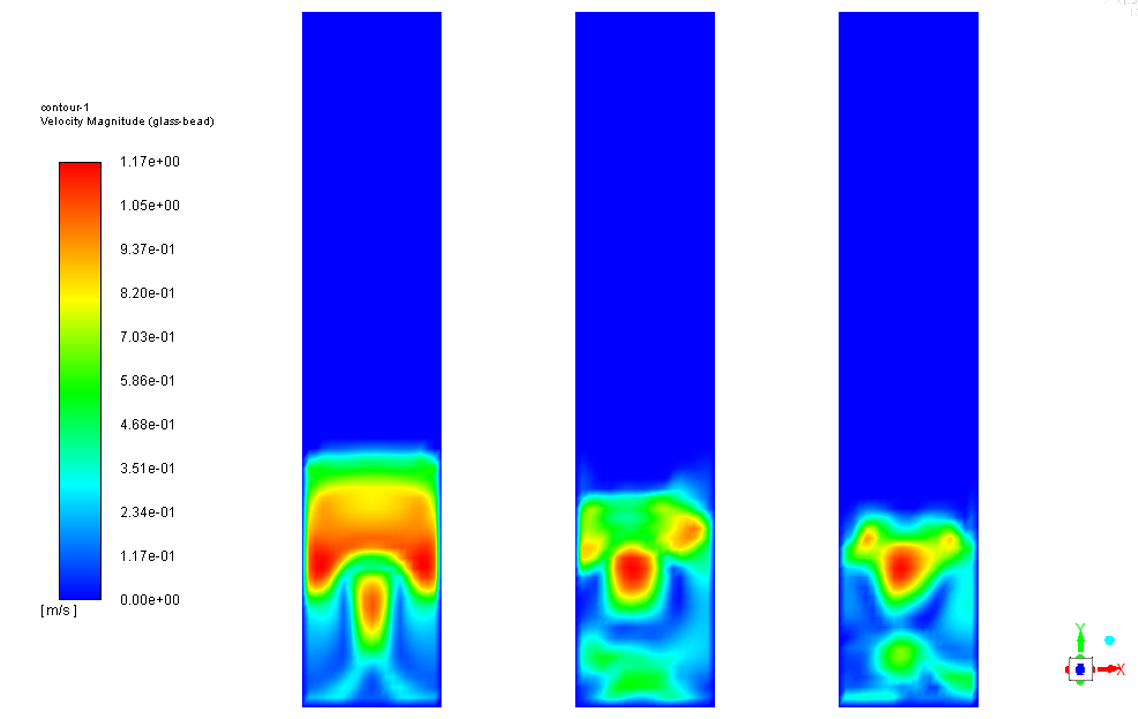
\includegraphics[width=0.9\linewidth,height=0.45\textheight,keepaspectratio]{velmag_1_736.png}\\
            {\scriptsize \textit{Moderate upward solid entrainment.}}
        \end{column}
        \begin{column}{0.48\textwidth}
            \centering
            \textbf{$U_g = 2.78$ m/s} \\
            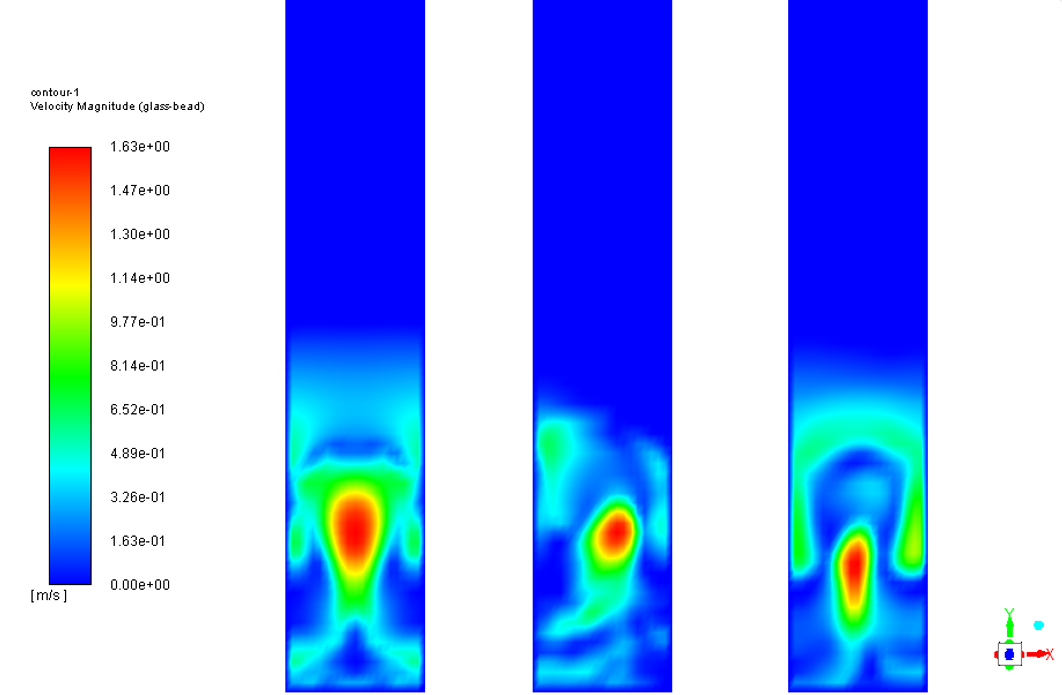
\includegraphics[width=0.9\linewidth,height=0.45\textheight,keepaspectratio]{velmag_2_78.png}\\
            {\scriptsize \textit{Enhanced solid circulation and mixing.}}
        \end{column}
    \end{columns}
    \vspace{0.3cm}
    \begin{block}{Particle Motion}
    Solids are dragged rapidly upwards in the wake of the bubbles and recirculate downwards near the walls. The higher gas velocity substantially increases the peak solid velocities and overall bed mixing.
    \end{block}
\end{frame}

\begin{frame}{Time Evolution at Monitored Probe}
    \begin{columns}[c]
        \begin{column}{0.48\textwidth}
            \centering
            \textbf{Probe Data ($U_g = 1.736$ m/s)}\\
            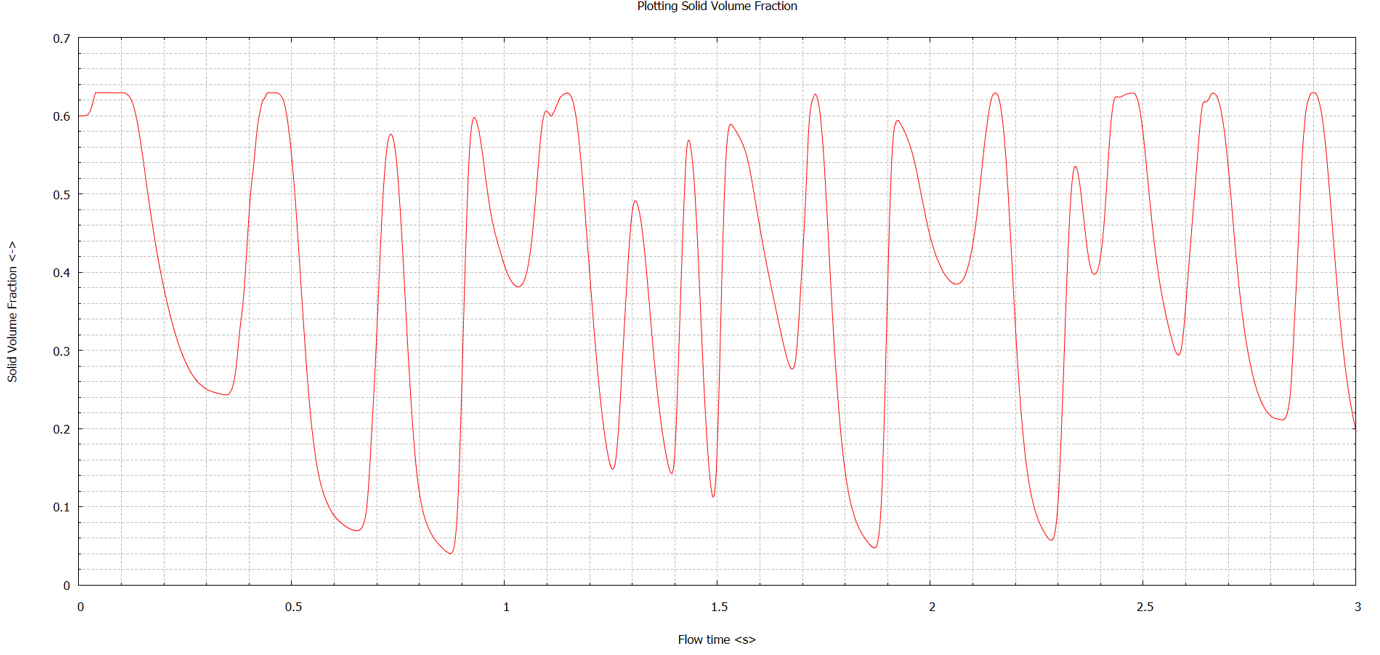
\includegraphics[width=\linewidth,height=0.25\textheight,keepaspectratio]{plot_volfrac_1_736.png} \\
            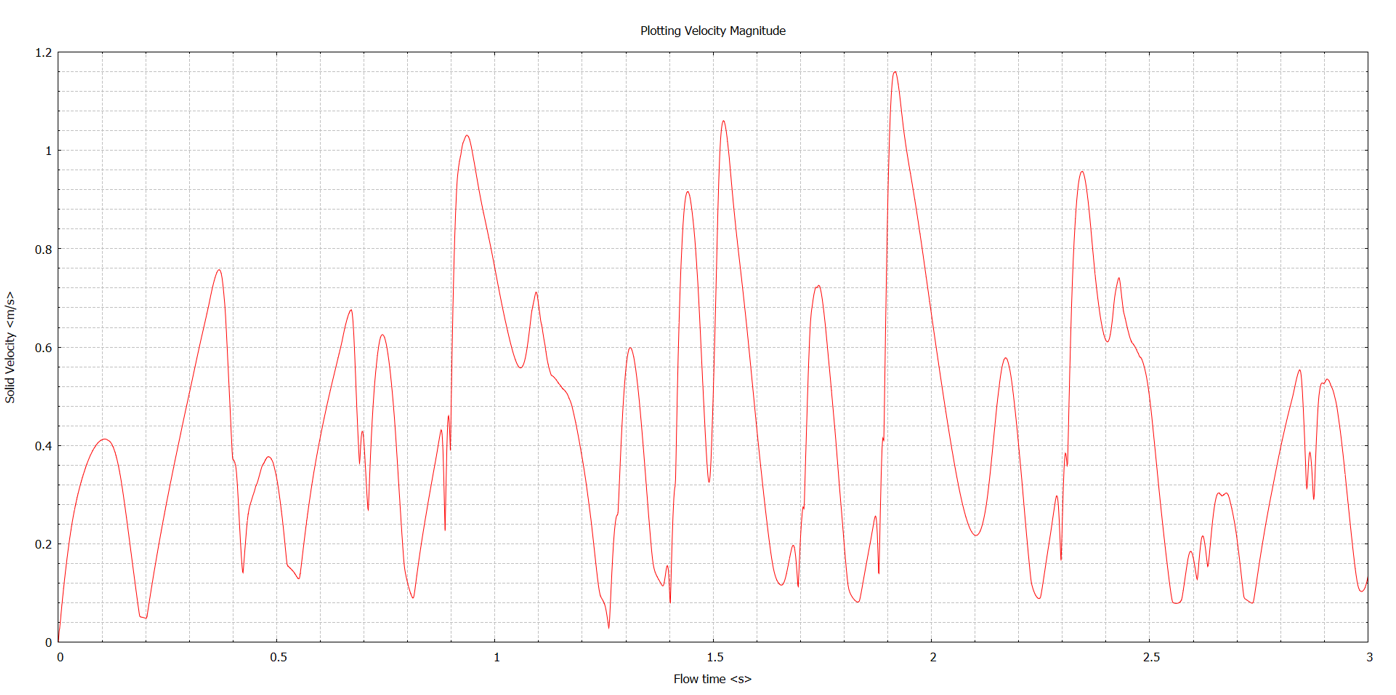
\includegraphics[width=\linewidth,height=0.25\textheight,keepaspectratio]{plot_vel_1_736.png}
        \end{column}
        \begin{column}{0.48\textwidth}
            \centering
            \textbf{Probe Data ($U_g = 2.78$ m/s)}\\
            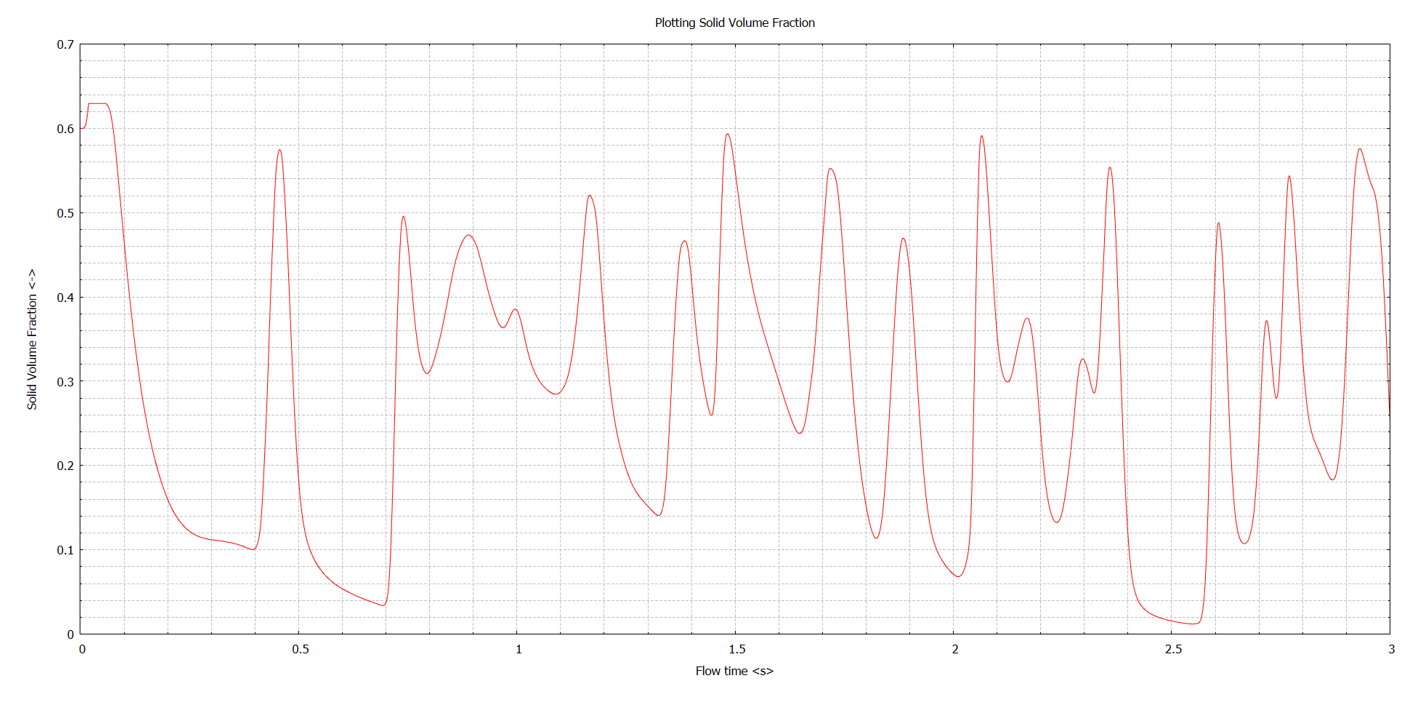
\includegraphics[width=\linewidth,height=0.25\textheight,keepaspectratio]{plot_volfrac_2_78.png} \\
            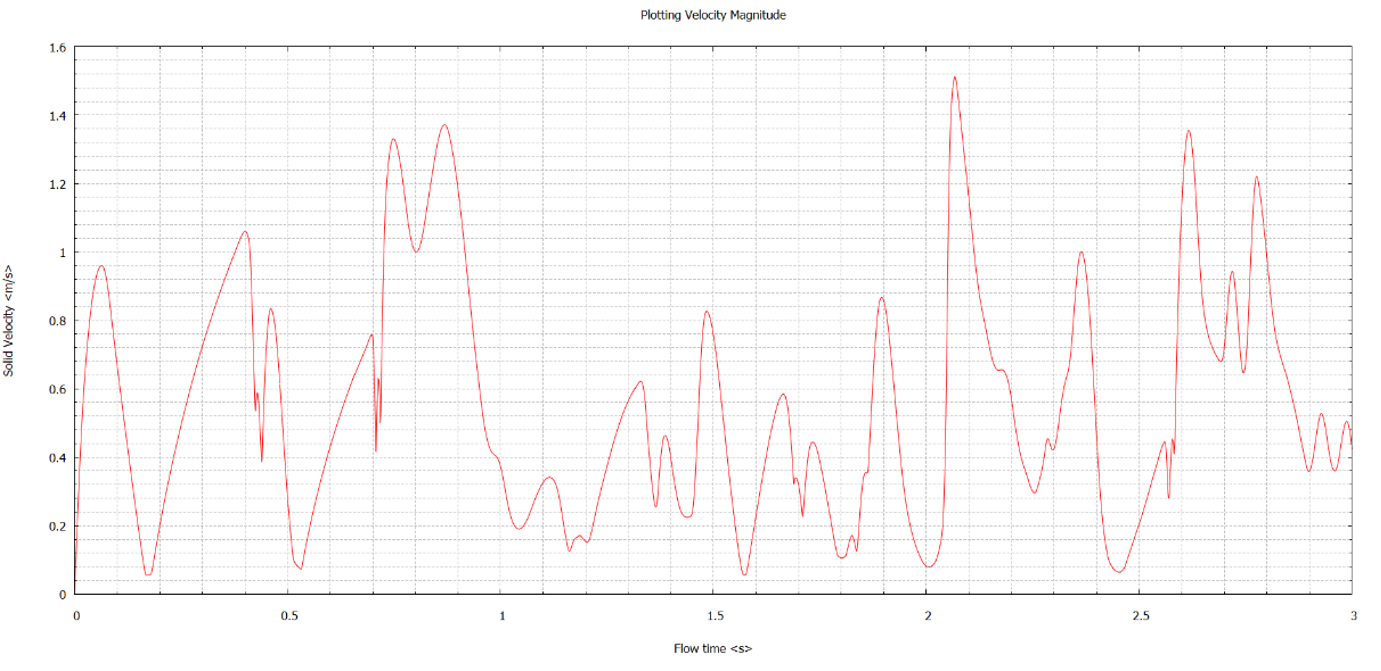
\includegraphics[width=\linewidth,height=0.25\textheight,keepaspectratio]{plot_vel_2_78.png}
        \end{column}
    \end{columns}
    \vspace{0.2cm}
    \begin{block}{Analysis at Fixed Point ($x=0.1, y=0.1$)}
    Sharp drops in $\alpha_s$ corresponding to spikes in solid velocity indicate the passing of a bubble through the probe location. The higher velocity case exhibits much higher frequency and intensity of bubbling.
    \end{block}
\end{frame}

% --- TUTORIAL 6 START ---
\section{Tutorial 6: Free Surface Flow (Bubble Rise)}
\begin{frame}
    \centering \Huge \textbf{Tutorial 6: Free Surface Flow (Bubble Rise)}
\end{frame}
\begin{frame}{Problem Statement \& Objective}
    \begin{block}{Objective}
    Perform 2D numerical simulations of a single air bubble rising in a quiescent liquid (water) using the Volume of Fluid (VOF) method.
    \end{block}
    \vspace{0.3cm}
    \begin{block}{System Details}
    \bi
        \im \textbf{Geometry:} Rectangular domain ($30$ mm width $\times$ $72$ mm height).
        \im \textbf{Initial Bubble:} $6$ mm diameter air bubble located $0.5$ diameters above the bottom wall.
        \im \textbf{Phases:} Primary: Water ($\rho=998.2$ kg/m$^3$, $\mu=0.0012$ kg/m-s). Secondary: Air ($\rho=1.225$ kg/m$^3$, $\mu=1.789\times 10^{-5}$ kg/m-s). Surface tension $\sigma = 0.072$ N/m.
    \ei
    \end{block}
\end{frame}

\begin{frame}{Computational Setup}
    \begin{columns}[T]
        \begin{column}{0.5\textwidth}
            \begin{block}{Boundary Conditions}
            \bi
                \im \textbf{Top Edge:} Pressure outlet ($0$ Pa gauge).
                \im \textbf{Side \& Bottom Edges:} Wall (No-slip).
            \ei
            \end{block}
            \begin{block}{Models}
            \bi
                \im \textbf{Multiphase Model:} Volume of Fluid (VOF), Explicit formulation.
                \im \textbf{Viscous Model:} Laminar.
            \ei
            \end{block}
        \end{column}
        \begin{column}{0.48\textwidth}
            \begin{block}{Numerical Schemes}
            \bi
                \im \textbf{Solver:} Pressure-based, Transient, Planar.
                \im \textbf{P-V Coupling:} PISO algorithm.
                \im \textbf{Spatial Discretization:} PRESTO! (Pressure), QUICK (Momentum).
                \im \textbf{Interface Reconstruction:} Geometric Reconstruction.
                \im \textbf{Transient Formulation:} 1st Order Implicit ($\Delta t = 10^{-5}$ s).
            \ei
            \end{block}
        \end{column}
    \end{columns}
\end{frame}

\begin{frame}{Geometry, Meshing \& Initial State}
    \begin{columns}[c]
        \begin{column}{0.48\textwidth}
            \centering
            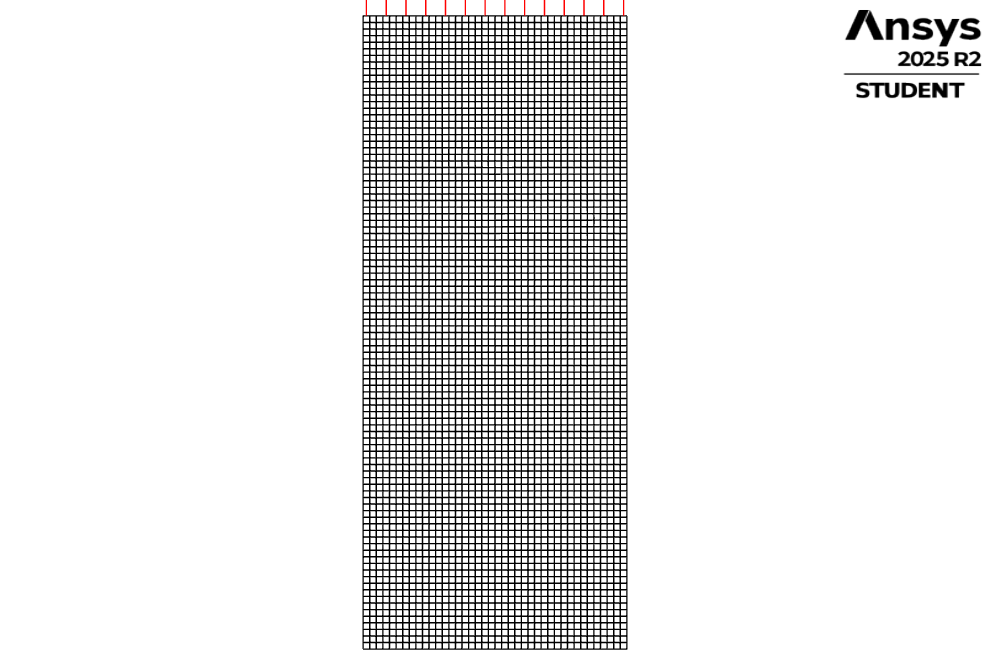
\includegraphics[width=0.6\linewidth,height=0.45\textheight,keepaspectratio]{tut6_mesh.png}\\
            \vspace{0.1cm}
            {\scriptsize \textit{Uniform grid ($0.75$ mm element size).}}
        \end{column}
        \begin{column}{0.48\textwidth}
            \centering
            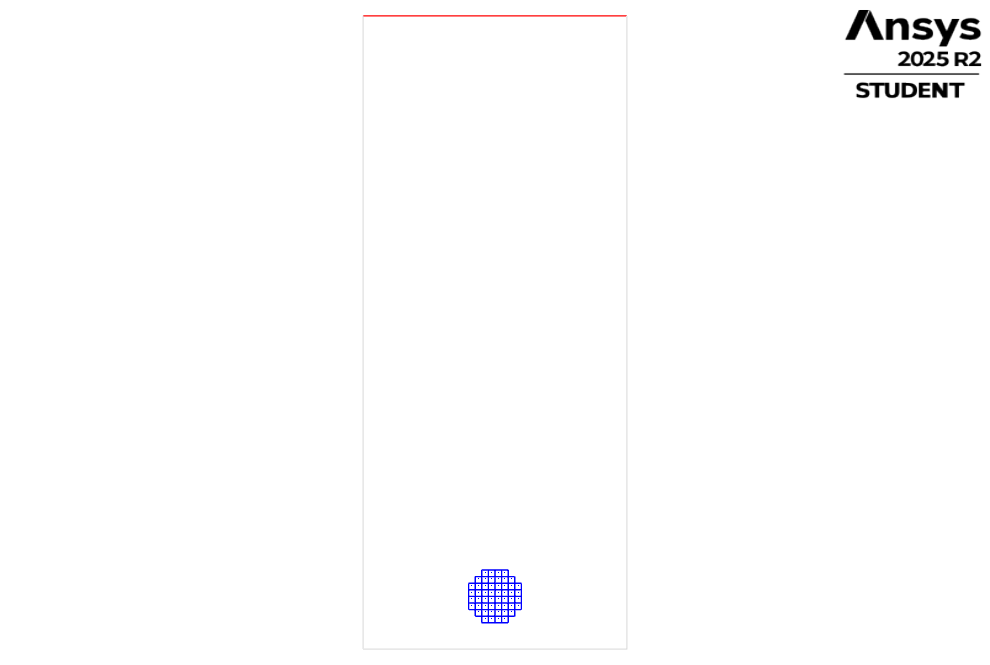
\includegraphics[width=0.8\linewidth,height=0.45\textheight,keepaspectratio]{tut6_bubble_patch.png}\\
            \vspace{0.1cm}
            {\scriptsize \textit{Initial bubble patch ($t=0$).}}
        \end{column}
    \end{columns}
    \vspace{0.2cm}
    \begin{block}{Mesh \& Initialization}
    A uniform grid was used to ensure $8$ cells per bubble diameter ($6\text{ mm}/8 = 0.75\text{ mm}$). The air bubble was initialized by patching a circular region with a volume fraction of $1$.
    \end{block}
\end{frame}

\begin{frame}{Bubble Deformation (VOF Tracking)}
    \begin{columns}[c]
        \begin{column}{0.24\textwidth}
            \centering
            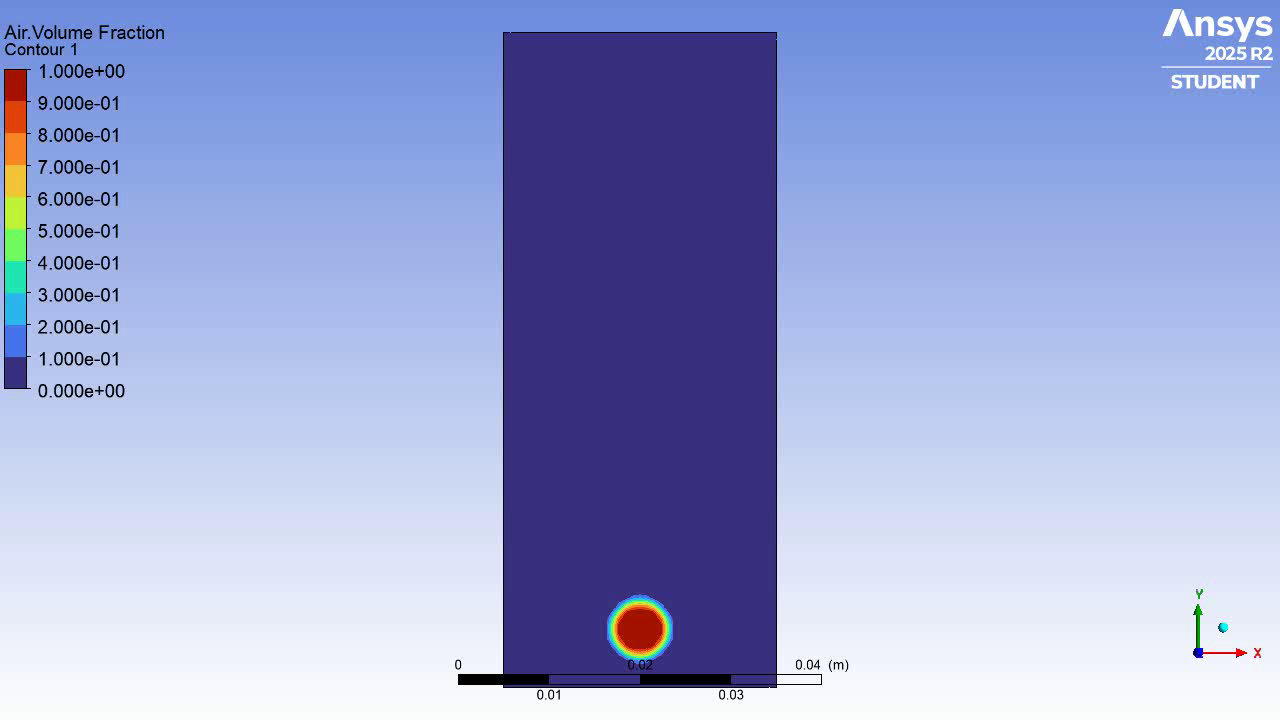
\includegraphics[width=\linewidth,height=0.45\textheight,keepaspectratio]{tut6_bubble_t1.png}
        \end{column}
        \begin{column}{0.24\textwidth}
            \centering
            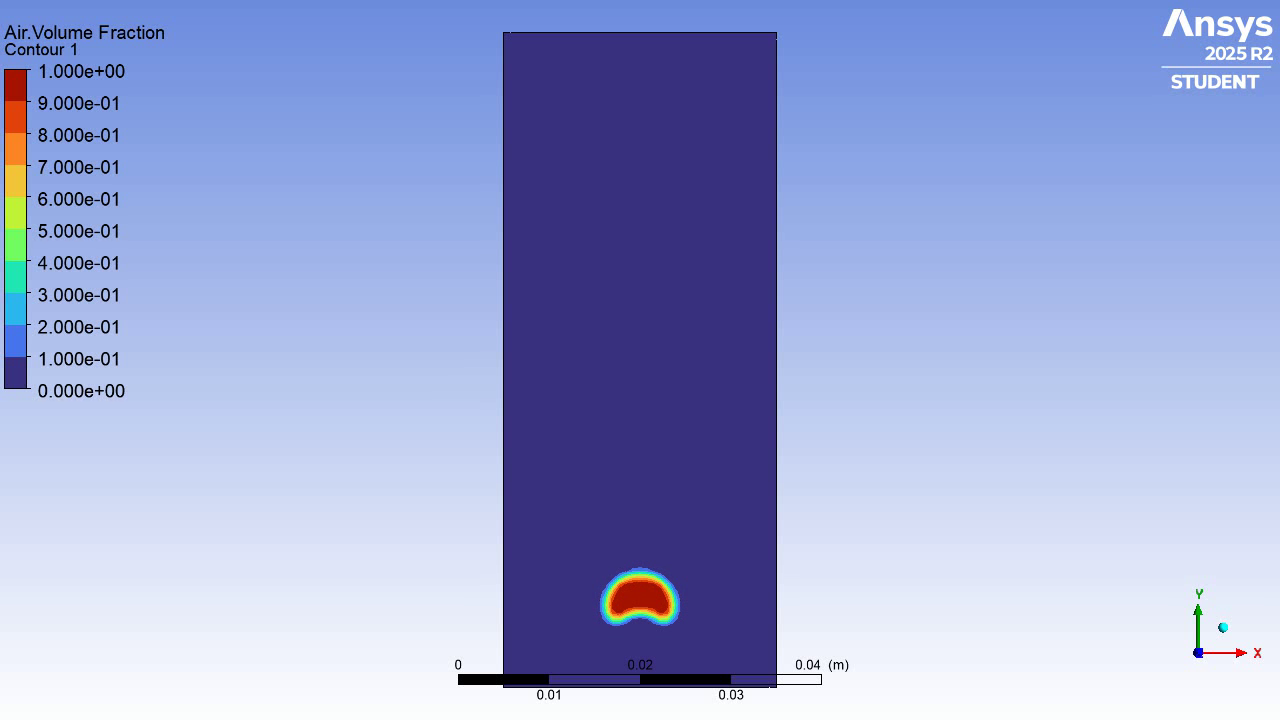
\includegraphics[width=\linewidth,height=0.45\textheight,keepaspectratio]{tut6_bubble_t2.png}
        \end{column}
        \begin{column}{0.24\textwidth}
            \centering
            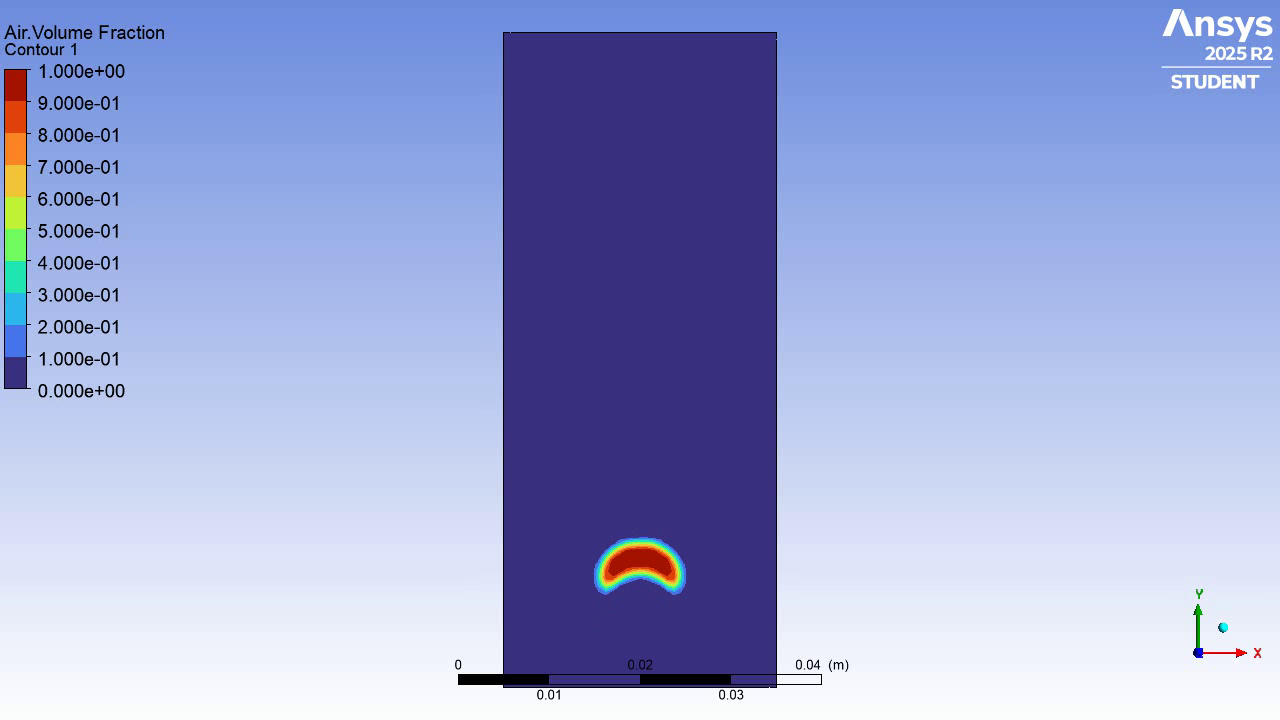
\includegraphics[width=\linewidth,height=0.45\textheight,keepaspectratio]{tut6_bubble_t3.png}
        \end{column}
        \begin{column}{0.24\textwidth}
            \centering
            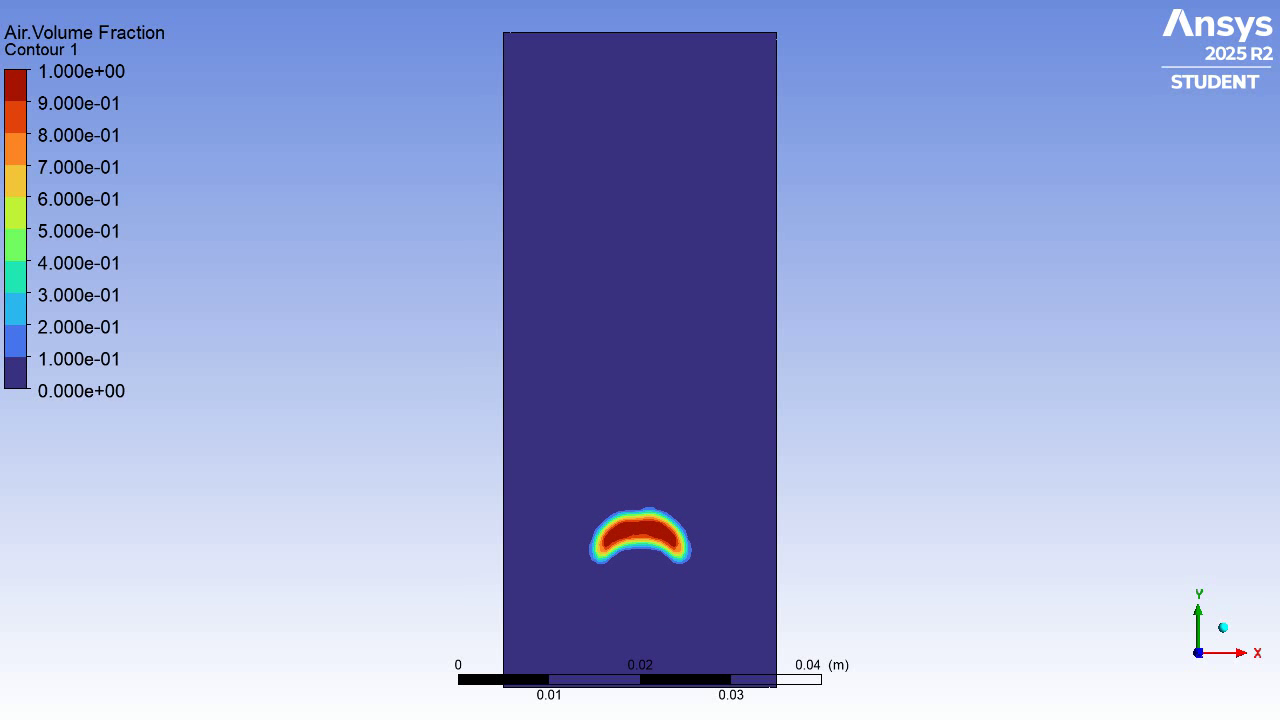
\includegraphics[width=\linewidth,height=0.45\textheight,keepaspectratio]{tut6_bubble_t4.png}
        \end{column}
    \end{columns}
    \vspace{0.2cm}
    \begin{block}{Transient Rise Dynamics}
    \small
    The VOF method and Geometric Reconstruction scheme successfully capture the interface deformation over time. The bubble transitions from its initial spherical shape into a dimpled/skirted shape due to hydrodynamic forces dominating over surface tension, consistent with the Clift et al. bubble shape regimes. \\
    \vspace{0.2cm}
    \textbf{Watch Animation:} \href{https://github.com/sajeev505/cll769_tuts_submission/blob/main/Tut_6/video.avi}{Click here to view the bubble rise video on GitHub!}
    \end{block}
\end{frame}

\end{document}